% CVPR 2022 Paper Template
% based on the CVPR template provided by Ming-Ming Cheng (https://github.com/MCG-NKU/CVPR_Template)
% modified and extended by Stefan Roth (stefan.roth@NOSPAMtu-darmstadt.de)

\documentclass[10pt,twocolumn,letterpaper]{article}

%%%%%%%%% PAPER TYPE  - PLEASE UPDATE FOR FINAL VERSION
%\usepackage[review]{cvpr}      % To produce the REVIEW version
\usepackage{cvpr}              % To produce the CAMERA-READY version
%\usepackage[pagenumbers]{cvpr} % To force page numbers, e.g. for an arXiv version

% Include other packages here, before hyperref.
\usepackage{graphicx}
\usepackage{amsmath}
\usepackage{amssymb}
\usepackage{booktabs}

% It is strongly recommended to use hyperref, especially for the review version.
% hyperref with option pagebackref eases the reviewers' job.
% Please disable hyperref *only* if you encounter grave issues, e.g. with the
% file validation for the camera-ready version.
%
% If you comment hyperref and then uncomment it, you should delete
% ReviewTempalte.aux before re-running LaTeX.
% (Or just hit 'q' on the first LaTeX run, let it finish, and you
%  should be clear).
\usepackage[pagebackref,breaklinks,colorlinks]{hyperref}


% Support for easy cross-referencing
\usepackage[capitalize]{cleveref}
\crefname{section}{Sec.}{Secs.}
\Crefname{section}{Section}{Sections}
\Crefname{table}{Table}{Tables}
\crefname{table}{Tab.}{Tabs.}


%%%%%%%%% PAPER ID  - PLEASE UPDATE
\def\cvprPaperID{Milestone 1} % *** Enter the CVPR Paper ID here
\def\confName{Stanford CS231N}
\def\confYear{2023}


\begin{document}

%%%%%%%%% TITLE - PLEASE UPDATE
\title{\\Exploring Robustness of Stanford's DeepSolar to Distribution Shifts}

% For a paper whose authors are all at the same institution,
% omit the following lines up until the closing ``}''.
% Additional authors and addresses can be added with ``\and'',
% just like the second author.
% To save space, use either the email address or home page, not both

\author{Kerrie Wu \\
  Stanford University \\
  {\tt\small kerriewu@stanford.edu} \\
  % Examples of more authors
   \and
    Julian Cooper \\
  % ICME \\
  Stanford University \\
  \tt\small {jelc@stanford.edu} \\
   \and
   Andrea van den Haak \\
  % ICME \\
  Stanford University \\
  \tt\small {vandenhaak@stanford.edu} \\
}
\maketitle

% %%%%%%%%% ABSTRACT
% \begin{abstract}
% \end{abstract}

%%%%%%%%% BODY TEXT
\section{Introduction}
\label{sec:intro}

We are interested in segmenting and classifying rooftop solar panels from satellite images, with a focus on residential areas. In many countries (including the United States), the rollout of rooftop solar has been ad hoc and largely untracked. Besides industrial sites and city buildings, electricity utilities are largely blind to where and how much solar neighborhoods have accumulated. Being able to estimate this (and its rate of increase) allows utilities to predict power output reasonably well (from meteorology forecasts) and adjust grid management and investment. \cite{Kasmi2023}

\section{Problem Statement}
Stanford's DeepSolar team have largely solved this challenge for the United States \cite{DeepSolar1} \cite{DeepSolar2}. However there are two major ways that the model can be improved: (1) segmentation accuracy and (2) robustness to distribution shifts.

The original DeepSolar model has two branches, a classification branch that detects if there is a solar panel in an image, and a segmentation branch that produces a class activation map based on the image, which can be used to estimate the total area of solar panels in the image if the classification branch predicts positive \cite{DeepSolar1}. The output class activation map is much lower in resolution than the input image size in the model, which means the segmentation is approximate and limited in detail. If the segmentation is more accurate and at the same resolution as the input, it could be used to predict the type of solar panel, and generate a more accurate estimate of the solar panel area. Therefore we seek to improve the resolution of the segmentation branch in our project.

Secondly, the DeepSolar model is not robust to "distribution shifts". This means that the model accuracy drops when tested on datasets from other regions with different satellite imagery to its USA-based training data. With the help of the DeepSolar team, we investigate different techniques for modifying the DeepSolar segmentation model in order to improve its robustness to distribution shifts. This will enhance the model's generalizability for use in countries other than the United States by requiring less (or ideally zero!) labeled data from other countries for finetuning the model.

%-------------------------------------------------------------------------

\section{Literature Review}
 
We are looking into augmenting the segmentation branch of the model to produce more accurate segmentation outputs by incorporating Facebook's Segment Anything Model \cite{kirillov2023segment}. The Segment Anything Model is a foundational transformer vision model capable of zero-shot image segmentation, given an input image and point prompts of portions of the image to include, or exclude, in the mask. We anticipate that due to its extensive pretraining, we can use it to produce accurate segmentation masks for solar PV arrays that are the same size as the original input image without any finetuning.

In addition to incorporating the Segment Anything Model, we have also reviewed several papers on techniques for measuring robustness to and handling distribution shift. 

\begin{itemize}
    \item Taori, 2020 \cite{Taori2020}: Major contributions included defining effective robustness and relative robustness metrics. The authors also concluded that robustness to synthetic data distribution shifts do not imply robustness to natural distribution shifts, and that a more diverse training set improved robustness.
    \item Yao, 2022 \cite{yao2022improving}: Describes a data augmentation method called LISA adds interpolations between original input-output training example pairs to the training data. The interpolation pairs can be selected in a targeted manner to improve robustness to domain shifts.
    \item Volpi, 2018 \cite{volpi2018generalizing}: Describes how to adversarially augment the training data to achieve a more robust model. At each training iteration, the training examples fed to the model are augmented with examples that are considered difficult for the current model.
\end{itemize}

\section{Data Set}

We make use of two satellite imagery datasets for this project: (1) the original Deepsolar United States dataset, published in 2017 \cite{DeepSolar1}, and (2) a recently published dataset for France (released January 2023) \cite{Kasmi2023}.  

The United States dataset is large and highly skewed. It includes 46,090 images with solar panels (positive) and 366,467 images without solar panels (negative). For positive images, we also have access to masks with 1 and 0 pixels indicating exactly where in the image the solar panel lies. The dataset covers most industrial and residential regions of the country.\cite{DeepSolar1} 

 The France dataset provides ground truth segmentation masks for 13,303 images from Google Earth25 and 7,686 images from the French national Institute of Geographical and Forestry Information (IGN). It includes no negative satellite images (no ability to perform classification) and focuses on more rural and residential regions. \cite{Kasmi2023} We will use this to test our model's ability to handle distribution shifts by training our model on United States data, but validating and testing our model on France data. \\


\section{Technical Approach}
Before starting our analysis, we needed to invest significant work in standing back up the DeepSolar model, including (1) rewriting some components from TensorFlow into PyTorch, (2) fixing bugs associated with out-dated APIs, (3) ensuring code could natively make use of GPU resources, (4) rebuild partially broken image processing pipeline, and (5) reproduce baseline figures to convince ourselves that any fixes had been properly implemented.

To incorporate the Segment Anything Model \cite{kirillov2023segment}, we adopt a similar data processing pipeline as the original DeepSolar Team \cite{DeepSolar1}. We feed an input image to the original DeepSolar classification/segmentation model. If the DeepSolar model's classification branch predicts positive, then we use the segmentation branch's output class activation map (CAM) to generate point prompts to SAM: three positive (to include in the mask), and three negative (to exclude from the mask). As an initial approach, we normalize the CAM map to values between 0 and 1, and randomly select three points where the scaled CAM value is above 0.5 as positive points, and three points where the CAM value is below 0.1 as negative points. To evaluate performance and compare to baseline, we will use intersection over union and percent error in estimated solar PV area. 

To handle the distribution shift between our United States and France datasets, we plan to experiment with interpolation-based data augmentation through LISA \cite{yao2022improving}, regularized fine-tuning \cite{li2021}, and adversarial data augmentation \cite{volpi2018generalizing}. To measure how well our model handles distribution shifts, we will use indsutry standard quantitative metrics such as effective robustness and relative robustness as defined by Taori \cite{Taori2020}. (Note, we include percent error in predicted solar PV area to measure segmentation model performance irrespective of robustness.) 


\section{Intermediate/Preliminary Results}
Table 1 summarizes our preliminary results as of the milestone deadline. The first row shows the baseline precision, recall, and area percentage error for both the United States and French datasets when using the pre-existing DeepSolar pretrained model. We confirm that for the United States test data, our results match those from the DeepSolar paper \cite{DeepSolar1}, with impressive classification results, but poor segmentation accuracy. This gives us confidence that our efforts to bring the codebase up-to-date in order to use modern packages was done correctly. 

Baseline performance on our France dataset was worse than expected, especially for classification. This may indicate significant opportunity to improve DeepSolar's ability to handle distribution shifts (known to be an issue), but at this point we suspect there is still a bug in how we process and pass the France data into our model pipeline. That said, for the few images that were correctly classified (and segmentation attempted), we actually achieve very reasonable segmentation. See example CAM segmentation in Figure 1. 

The second line of Table 1 illustrates our first results from trying to enhance the segmentation classifier of our DeepSolar model. While the results are not amazing, they are already a meaningful improvement from the baseline. See Figure 2 for visualizations of several example outputs. For improving usage of SAM, we can investigate different methods of picking point prompts. This can include changing the number of point prompts provided to SAM, and different selection methods (eg, tuning the CAM value thresholds, or sampling based on a probability distribution instead of randomly).


\begin{table*}[htp]

\begin{tabular}{||c | c | c | c | c | c | c | c  | c ||}
\hline
Model & \multicolumn{4}{c|}{US dataset} & \multicolumn{4}{c|}{French dataset} \\ [0.5ex] 
\hline\hline
{} & precision & recall & area \% error & IOU & precision & recall & area \% error & IOU \\ 
\hline
Deepsolar US (baseline) & 0.95 & 0.86 & -8.0\% & NA & 1.00 & 0.001 & 0.47\% & NA \\ 
\hline
Deepsolar US + SAM &  0.95 & 0.86 & 47.0 \% & 0.24 & TBD & TBD & TBD & TBD\\ 
\hline

\end{tabular}
\begin{center}

\caption{Preliminary results showing performance of the baseline model (Deepsolar US) on the original US dataset, compared to results with the same model on the French dataset. We also compare US dataset results to those of the original Deepsolar US model but using Facebook's Segment Anything Model for segmentation. Precision and Recall are both based on the image classification performance of the model (which are the same between the baseline and with SAM). Percent area error measures the percent difference between the predicted solar PV area and the true solar PV area as measured by the true segmentation masks. IOU stands for intersection over union and is calculated only for models using SAM because the CAM maps produced by the original Deepsolar model are lower resolution than the true segmentation labels, and therefore can't be used to calculate an IOU score. Future work includes adapting the DeepSolar Model to the French dataset and trying to use SAM on the French dataset to fill in the remaining TBD values in the table. }

\end{center}
\end{table*}

\begin{figure*}[htp]
\centering
\begin{subfigure}{.3\textwidth}
    \centering
    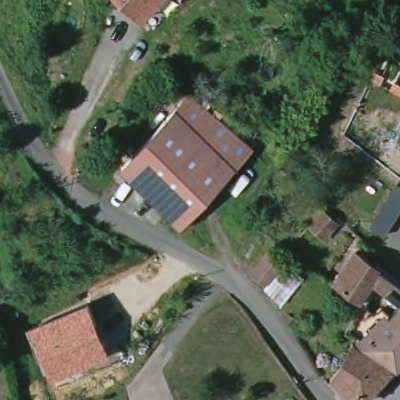
\includegraphics[width=.95\linewidth]{example.png}  
    \caption{Raw image}
    % \label{Raw image}
\end{subfigure}
\begin{subfigure}{.3\textwidth}
    \centering
    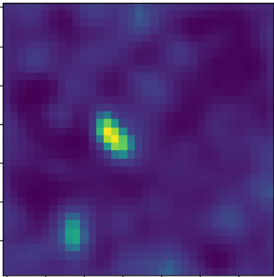
\includegraphics[width=.95\linewidth]{example_cam_seg.png}  
    \caption{CAM segmentation}
    % \label{CAM segmentation}
\end{subfigure}
\begin{subfigure}{.3\textwidth}
    \centering
    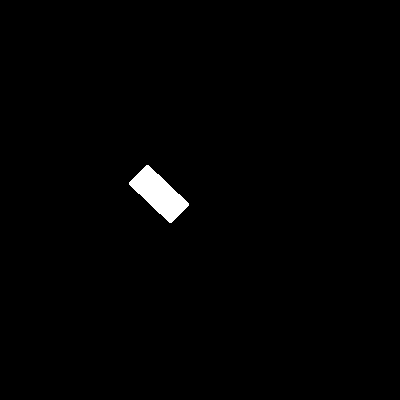
\includegraphics[width=.95\linewidth]{example_true_seg.png}  
    \caption{True segmentation}
    % \label{True segmentation}
\end{subfigure}
\caption{Example result from DeepSolar baseline model trained on United States data and asked to predict segmentation masks of France test image data. True segmentation masks (rightmost), CAM activations from the original DeepSolar model (middle), and the original input image (leftmost).}
\label{FIGURE LABEL}
\end{figure*}

\begin{figure*}[htp]
\centering
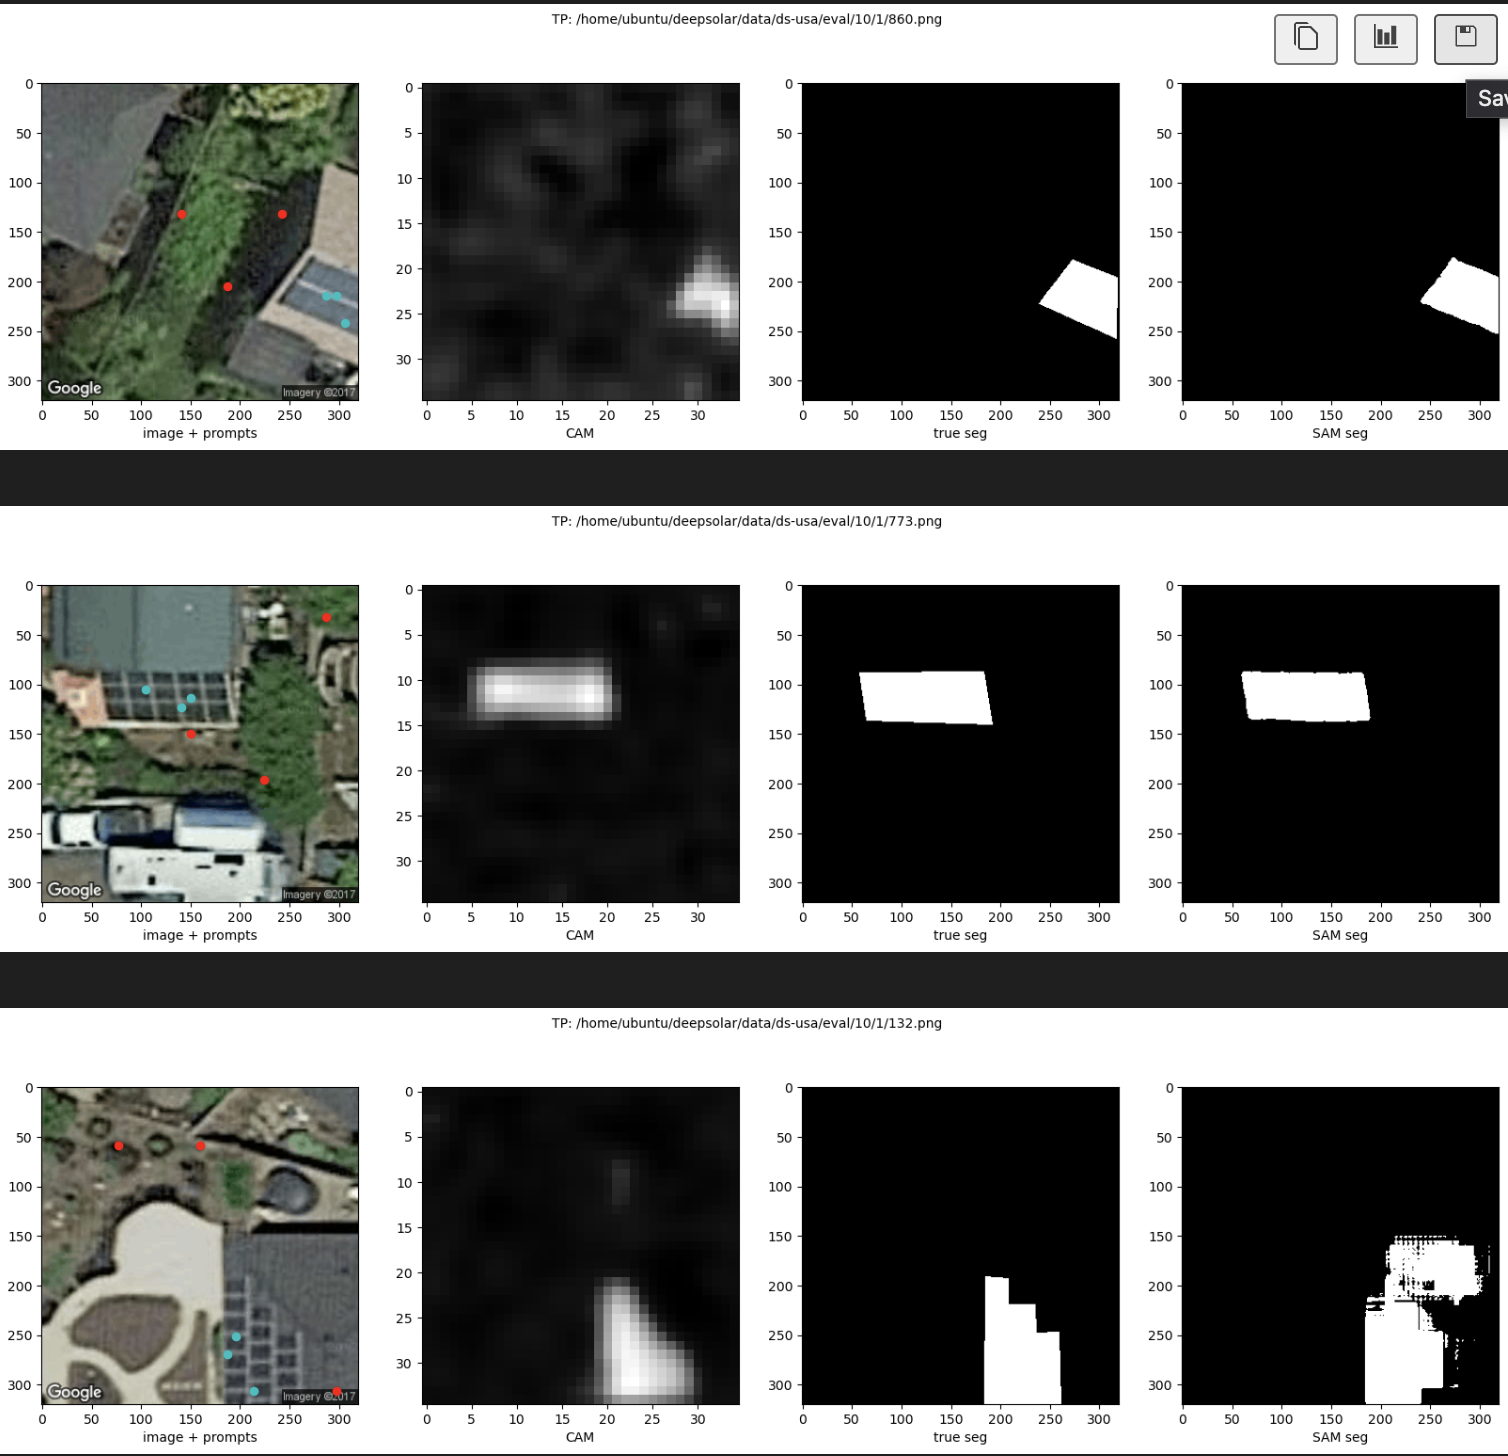
\includegraphics[width=15cm]{prelim_sam.png}
\caption{Preliminary segmentation of solar PV cells with SAM (rightmost column), compared to true segmentation masks (second from right), CAM activations from the original DeepSolar model (third from right), and the original input image (leftmost) with positive point prompts in cyan, and negative point prompts in red.}
\end{figure*}


%%%%%%%%% REFERENCES
\newpage
{\small
\bibliographystyle{ieee_fullname}
\bibliography{egbib}
}

\end{document}
